\documentclass[12pt]{article}

\usepackage[bottom = 15mm]{geometry}
\usepackage[utf8]{inputenc}
\usepackage[T2A]{fontenc}
\usepackage[russian]{babel}
\usepackage{graphicx}
\usepackage{caption}
\usepackage{amssymb, gensymb, amsmath}
\usepackage{mathrsfs}
\usepackage{array, colortbl}


\textwidth = 16 cm
\textheight = 23  cm
\oddsidemargin = 0 pt
\topmargin = -1.5 cm
\parindent = 20 pt
\parskip = 0 pt
\flushbottom


\title{{\bf Задача 3.\,4.\,2 \\ Закон Кюри-Вейсса}}
\author{Лось Денис (группа 611)}
\date{24 ноября 2017}



\begin{document}

\maketitle

\paragraph{Цель работы: } изучение температурной зависимости магнитной восприимчивости ферромагнетика выше точки Кюри.

\paragraph{В работе используются: } катушка самоиндукции с образцом из гадолиния, термостат, 	частотометр, цифровой вольтеметр, $LC$ автогенератор, термопара медь-константант.

\section*{Экспериментальная установка}
\par
	Схема установки для проверки закона Кюри-Вейсса показана на рис.1. Исследуемый ферромагнитный образец (гадолиний) расположен внутри пустотелой катушки самоиндукции, которая служит индуктивностью колебательного контура, входящего в состав $LC$ автогенератора.
\begin{figure}[h!]
	\centering
	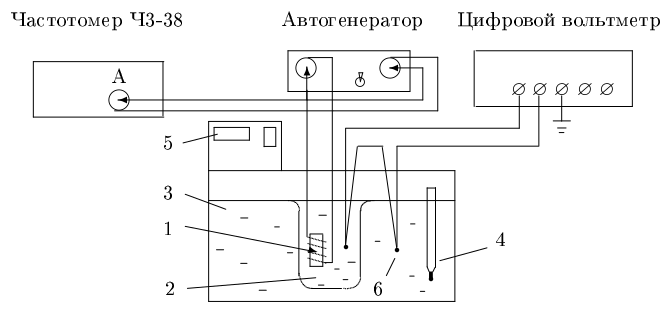
\includegraphics[width = 12cm, height=7cm]{image1.png}
	\caption{Схема экспериментальной установки}
\end{figure}
\par
	Катушка 1 с образцом помещена в стеклянный сосуд 2, залитый трансформаторным маслом. Масло предохраняет образец от окисления и способствует ухудшению электрического контакта между отдельными частиками образца. Кроме того, оно улучшает тепловой контакт между образцом и термостатируемой (рабочей) жидкостью 3 в термостате. Ртутный термометр 4 используется для приближённой оценки температуры. Температура образца регулируется с помощью термостата.
\par
	Магнитная восприимчивость образца $\chi$ определяется по изменению самоиндукции катушки. Обозначив через $L$ самоиндукцию катушки с образцом и через $L_0$ --- её самоиндукцию в отсутствие образца, получим
\[
	\left(L - L_0\right) \sim \chi
\]
При изменении самоиндукции образца меняется период колебаний автогенератора:
\[
	\tau = 2 \pi \sqrt{LC},
\]
где $C$ --- ёмкость контура автогенератора.	
\par
	Период колебаний в отсутсвие образца определяется самоиндукцией пустой катушки:
\[
	\tau_0 = 2 \pi \sqrt{L_0 C}
\]
В результате получим, что
\[
	\left(L - L_0\right) \sim \left(\tau^2 - \tau_0^2 \right)
\]
А следовательно,
\[
	\chi \sim \left(\tau^2 - \tau_0^2\right)
\]
Из приведённых формул следует, что закон Кюри-Вейсса справедлив, если выполнено соотношение
\[
	\frac{1}{\chi} \sim \left(T - \Theta_p\right) \sim \frac{1}{\left(\tau^2 - \tau_0^2 \right)}
\]
\par
	Измерения проводятся в интервале температур от $14 \, \degree \text{C}$ до $40 \, \degree \text{C}$. Температура исследуемого образца всегда несколько отличается от температуры дистиллированной воды в сосуде. После того как вода достигла заданной температуры, идёт медленный процесс выравнивания температур образца и воды. Разность их температур контрольриуется с помощью медно-константановой термопары 6 и цифрового вольтметра. Один из спаев термопары находится в тепловом контакте с образцом, а другой погружён в воду. Концы термопары подключены к цифровому вольтметру. Будем измерять период колебаний автогенератора в тот момент, когда указанная разность температур становится меньше $0.5 \, \degree \text{C}$ (более точному измерению мешают паразитные ЭДС, возникающие в цепи термопары).
	
\section*{Ход работы}
\par	
	Исследуем зависимость периода колебаний $LC$ генератора от температуры образца, отмечая период колебаний $\tau$ по частотометру, а температуру $T$ --- по показаниям дисплея и цифровому вольтметру ($\Delta U$ с учётом знака). Термопара у нас подключена так, что при знаке "+" на табло вольтметра температура образца выше температуры рабочей жидкости. Проведём измерения в диапазоне от $14 \, \degree \text{C}$ до $40 \, \degree \text{C}$ через $2 \, \degree \text{C}$ при нагревании и охлаждении.	
\begin{table}[h!]
	\centering
	\begin{tabular}{|c|c|c|c|}
	\hline
	$T_\text{жд}$, ${\degree \text{C}}$ & $\Delta U$, мкВ & $\tau$, мкc & $T$, $\degree \text{C}$ \\
	\hline	
	15&	1&	10.035&	15.02 \\
	\hline
	17&	13&	9.885&	17.31 \\
	\hline
	19&	17&	9.625&	19.41 \\
	\hline
	21&	11&	9.211&	21.26 \\
	\hline
	23&	15&	8.859&	23.36 \\
	\hline
	25&	15&	8.665&	25.36 \\
	\hline
	27&	12&	8.568&	27.29 \\
	\hline
	29&	15&	8.511&	29.36 \\
	\hline
	31&	15&	8.473&	31.36 \\
	\hline
	33&	15&	8.444&	33.36 \\
	\hline
	35&	13&	8.422& 	35.31 \\
	\hline
	37&	11&	8.405	& 37.26 \\
	\hline
	39&	12&	8.392 &	39.29 \\
	\hline
	\hline
	37	&15&	8.401&	37.36 \\
	\hline
	34	&16	&8.426&	34.38 \\
	\hline
	32	&17	&8.448&	32.41 \\
	\hline
	30&	17	&8.478&	30.40 \\
	\hline
	\end{tabular}	
\end{table}
\par
	В данной экспериментальной установке постоянная термопары $k = 24 \, \text{град/мВ}$, а период колебаний в отсутсвие образца $\tau_0 = 8.252 \, \text{мкс}$.
\begin{figure}[h!]
	\centering
	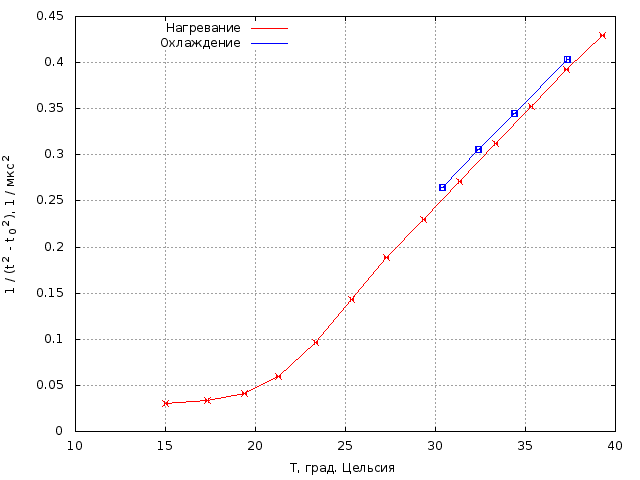
\includegraphics[height = 7cm, width = 12cm]{plot1.png}
	\caption{График зависимости $1 \, / \left(\tau^2 - \tau_0^2\right) = f(T)$}
\end{figure}
\newpage
\par
	Построив график зависимости $1 / \left(\tau^2 - \tau_0^2\right) = f(T)$ и экстраполировав полученный график к оси абсцисс, найдём парамагнитную точку Кюри для гадолиния. В результате получим, что
\[
	\Theta_p = \left(18.1 \pm 0.5 \right) \, \degree \text{C}
\]
\end{document}
